\clearpage
\setcounter{page}{1}
\begin{appendix}

\section{Overview}
In the supplementary materials, we provide detailed information on the generation of the two datasets used for training HMFlow and HBSeg, along with corresponding benchmarks and evaluation metrics to facilitate their use and assessment in future research. Additionally, we include the implementation details of the Tokenizer in both Self-learning and Fine-tuning stages. For more comprehensive and extensive comparisons, we have expanded our comparison experiments on HuCenLife~\cite{xu2023human} to include methods tailored for modeling dynamic point cloud videos, to demonstrate the superiority of our method in capturing human motion representations. Finally, we also provide additional details regarding the size of the UniPVU-Human model and comparisons with others.
\section{Human Motion Flow (HMFlow)}
\label{sec:hmflow}
\subsection{Implementation Details}
\begin{figure}[ht]
    \centering
    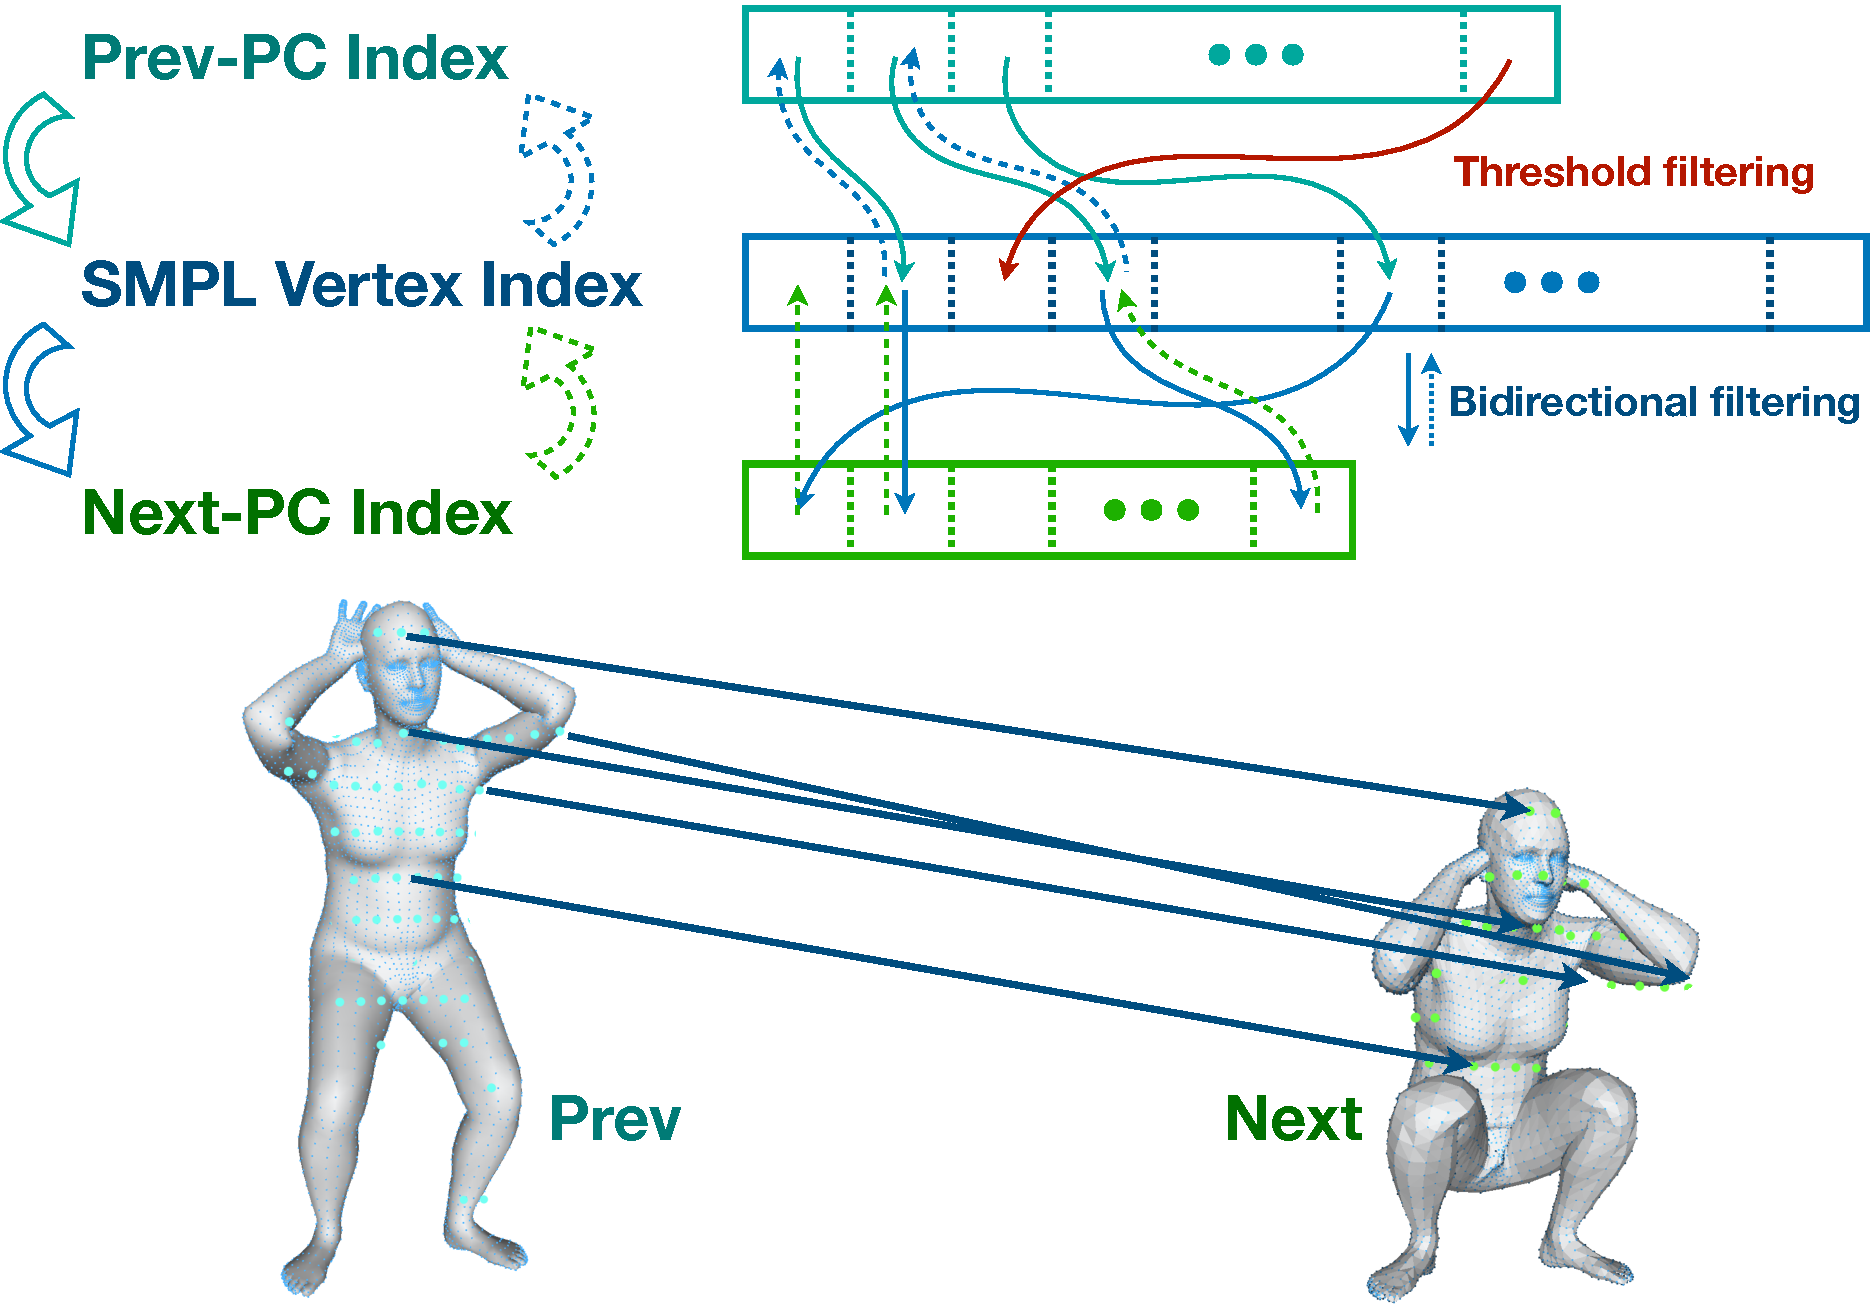
\includegraphics[width=1\columnwidth]{sup_pic/flow.pdf}
    \caption{The pipeline of generating the flow from the previous point cloud to the next point cloud. We associate each synthetic LiDAR point to its nearest SMPL vertex, to establish the correspondence between synthetic LiDAR points across different frames by using SMPL vertices indices as medium, so that we can obtain point-wise motion flow.}
    \label{fig:flow}
    \vspace{-1ex}
\end{figure}
Due to rotation or occlusion, point clouds may flow in and out between consecutive frames, resulting in a lack of temporal correspondence. But for the SMPL~\cite{loper2023smpl} mesh, each mesh vertex can be matched between consecutive frames using vertex index. Therefore, we make a large-scale synthetic dataset, LiDARFlow-Human, by scanning the SMPL mesh surfaces of consecutive frames using a simulated LiDAR to generate simulated LiDAR point clouds (As shown in Figure.~\ref{fig:flow}). Each simulated LiDAR point is matched with its nearest SMPL vertex. Consequently, we use SMPL vertices as a medium to match simulated LiDAR points between frames. By subtracting coordinates, we obtain the point-wise motion flow. Moreover, we set a threshold to filter the distance and build the bidirectional connections to ensure the accuracy of the matching. Specifically, when the nearest distance from vertex to point is smaller than the defined threshold $D$, we think them has the unidirectional connection and we select the unidirectional connection $C_{p2n}$ from previous point cloud to next point clouds, meanwhile we select the unidirectional connection $C_{n2p}$ from next point clouds to previous point clouds. The bidirectional filter are used to delete the unidirectional connection without coincidence, $$Flow_{p2n} = C_{p2n}\cap{C_{n2p}}.$$


% We generate the point-wise motion flow depending on the SMPL vertices. As shown in Figure.~\ref{fig:flow}, the point clouds lack a specific order while the SMPL vertices are ordered temporally. Given that our point clouds possess corresponding SMPL parameters, we generate the SMPL vertices with the full parameters, which completely match with point clouds. Since the SMPL vertices maintain a consistent order, we use these vertices to connect the previous and next point cloud. The connections are established by distance, with each point being paired with its nearest vertex. Moreover, we set a threshold to filter the distance and we build the bidirectional connections to ensure the accuracy of the connections between the previous point cloud and the next point cloud.

% We generate the flow of point clouds depending on the SMPL mesh vertex. As shown in Figure.~\ref{fig:flow}, The point clouds are unordered while the SMPL vertex is ordered, and our point clouds have corresponding SMPL parameters, so we generate the SMPL mesh with the full parameters, which completely matches with point cloud. As the SMPL vertex is in the same order, we use the SMPL vertex to connect the previous and next point cloud. We build the connection by distance, each point has a paired nearest vertex. Moreover, we set a threshold to filter the distance and we build the bidirectional connection to ensure the accuracy of the connection between the previous point cloud and the next point cloud.

\subsection{Dataset and Evaluation Metrics}
We will contribute LiDARFlow-Human, used for training Human Motion Flow Estimator (HMFlow), to the community with corresponding benchmarks. As shown in Table.~\ref{tab:lidarflow_human}, we adopt the evaluation metrics used in ~\cite{puy2020flot,gu2019hplflownet,liu2019flownet3d,wu2019pointpwc}:
\begin{itemize}
\item EPE: End Point Error (meters). $$EPE = \frac{\sum_{i=1}^N \left\| (\vec{(f_{predict})_i}-\vec{(f_{gt})_i}) \right\|_2}{N},$$ where $\vec{(f_{predict})_i}$ and $\vec{(f_{gt})_i}$ are point-wise predicted motion flow and ground truth motion flow, respectively.

\item acc\_strict: percentage of points such that $EPE_i<0.05$ or $EPE_i/ \|\vec{f_i}\|_2<0.05$.
\item acc\_relax: percentage of points such that $EPE_i<0.1$ or $EPE_i/ \|\vec{f_i}\|_2<0.1$.
\item outlier: percentage of points such that $EPE_i>0.3$ or $EPE_i/ \|\vec{f_i}\|_2>0.1$.
\end{itemize}

% The above metrics are computed as follows. The point clouds $\vec{p}, \vec{q}$ are obtained by selecting $n$ random points out of the $N$ provided points in the datasets. The flow is estimated and compared to the ground truth flow $\vec{f}$ on these $n$ selected points. The scores are averaged over the whole validation/test set.
\section{Human Body Segmentation (HBSeg)}

\begin{figure}[t]
    \centering
    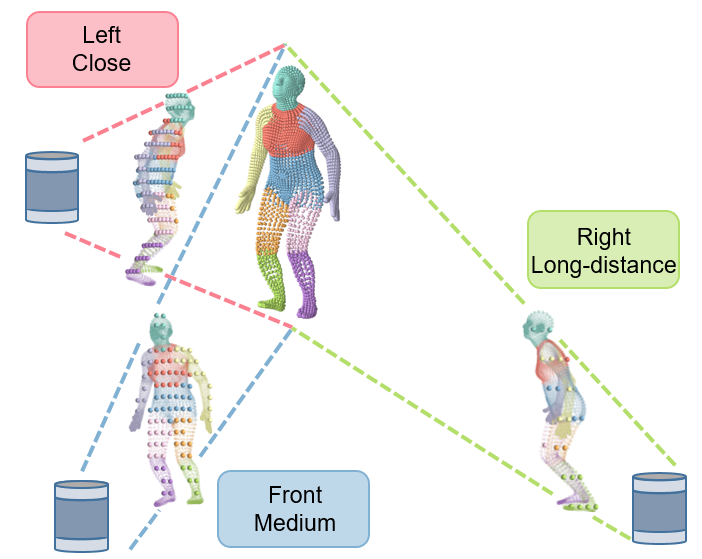
\includegraphics[width=1\columnwidth]{sup_pic/SMPL_1.png}
    \caption{We create a synthetic dataset of 1 million LiDAR human point cloud instances, using the AMASS dataset for 3D human meshes and simulating LiDAR scans from various perspectives and distances for enhancing the diversity of the samples, so as to better simulate the distribution of real-world data. } 
    \label{fig:HBSeg}
    \vspace{-1ex}
\end{figure}

\begin{table}[t]
\caption{Human Motion Flow (HMFlow) Result on LiDARFlow-Human.}
\label{tab:lidarflow_human}
\scalebox{0.95}{
\begin{tabular}{c|c|c|c|c}
\Xhline{1px}
     & EPE$\downarrow$    & acc\_strict$\uparrow$ & acc\_relax$\uparrow$ & outlier$\downarrow$ \\ \hline
FLOT~\cite{puy2020flot} & 0.14 & 83.67             & 95.77           & 0.78  \\ \Xhline{1px}
\end{tabular}
}
\end{table}

\begin{table*}[]\footnotesize
\centering
\caption{Human Body Segmentation (HBSeg) Results on LiDARPart-Human.}
\label{tab:lidarpart_human}
\begin{tabular}{c|c|c|c|c|c|c|c|c|c|c}
\Xhline{1px}
           & head & left-arm & right-arm & up-body & low-body & upleft-leg & upright-leg & lowleft-leg & lowright-leg & mIoU$\uparrow$ \\ \hline
PointNet~\cite{qi2017pointnet}   & 88.2 & 51.2     & 46.6      & 52.1    & 62.6     & 45.8       & 36.2        & 67.4        & 60.2         & 56.7 \\ \hline
PointNet++~\cite{qi2017pointnet++} & 88.6 & 69.5     & 69.9      & 65.4    & 82.2     & 82.7       & 82.5        & 89.1        & 89.4         & 79.9 \\ \hline
PointMLP~\cite{ma2022rethinking}   & 92.0 & 76.1     & 75.2      & 76.7    & 88.0     & 86.3       & 85.8        & 92.8        & 92.3         & 85.0 \\ \hline
PointNeXt~\cite{qian2022pointnext}  & 95.1 & 82.7     & 81.9      & 83.1    & 91.9     & 91.2       & 90.8        & 96.1        & 96.0         & \textbf{89.9} \\ \Xhline{1px}
\end{tabular}
\end{table*}


\begin{table*}[]\scriptsize
\centering
\caption{Supplementary Comparison Experiments on HuCenLife~\cite{xu2023human}. "DM" stands for "Dynamic Method," indicating whether it is a method used for modeling dynamic point cloud videos. For the static methods, which are designed for processing static point clouds, we apply them on each frame of the point cloud sequence and then fuse these frame features after the encoder network by element-wise adding. "SL" stands for "Self-learning", signifying whether the method employs a self-learning mechanism.}
\label{tab:sup_comp_exp}.
\scalebox{0.91}{
\begin{tabular}{l|l|l|c|c|c|c|c|c|c|c|c|c|c|c|c}
\Xhline{1px}
                                                          & DM                                                 & SL                                                 & lift & carry & move & pull\_push & sco-bal & hum-inter & fitness & entertain & sports & bend-over & sit  & walk-stand & mAcc \\ \hline
PointNet~\cite{qi2017pointnet}      & \textcolor{red}{\XSolidBrush} & \textcolor{red}{\XSolidBrush} & 45.5 & 48.8  & 33.3 & 84         & 59.4    & 2.6       & 65.3    & 49.3      & 34.8   & 29.2      & 54.3 & 61         & 47.3 \\ \hline
PointNet++~\cite{qi2017pointnet++}  & \textcolor{red}{\XSolidBrush} & \textcolor{red}{\XSolidBrush} & 49.5 & 45.7  & 35.6 & 52.7       & 59      & 6         & 28.6    & 43.8      & 41.2   & 31.9      & 38.8 & 55         & 40.7 \\ \hline
PointMLP~\cite{ma2022rethinking}    & \textcolor{red}{\XSolidBrush} & \textcolor{red}{\XSolidBrush} & 48.5 & 47.7  & 57.7 & 80.1       & 80.3    & 36.1      & 75.7    & 60.8      & 39.5   & 54.9      & 55.8 & 59.7       & 58.1 \\ \hline
PointNeXt~\cite{qian2022pointnext}  & \textcolor{red}{\XSolidBrush} & \textcolor{red}{\XSolidBrush} & 48.1 & 56.6  & 34.1 & 80         & 85.6    & 22.6      & 50      & 38        & 25.7   & 25.5      & 63.1 & 70.9       & 50   \\ \hline
PCT~\cite{guo2021pct}               & \textcolor{red}{\XSolidBrush} & \textcolor{red}{\XSolidBrush} & 39.7 & 54.9  & 52.3 & 80.2       & 89.8    & 9.8       & 63.3    & 73.6      & 37.7   & 62.5      & 51   & 75.8       & 57.6 \\ \hline
HuCenLife~\cite{xu2023human}        & \textcolor{red}{\XSolidBrush} & \textcolor{red}{\XSolidBrush} & 45   & 44.4  & 52.7 & 81.2       & 86.7    & 23.1      & 81.2    & 54.8      & 41.7   & 54.8      & 53.2 & 70         & 57.4 \\ \hline
PSTNet~\cite{fan2022pstnet}         & \textcolor{green}{\checkmark} & \textcolor{red}{\XSolidBrush} &30.2	&22.6&	61.4&	64.7&	74.6	&21.6&	20.8&	82.4&	39.7	&51.1&	36	&15.4&	43.4 \\ \hline
PSTNet++~\cite{fan2021deep}         & \textcolor{green}{\checkmark} & \textcolor{red}{\XSolidBrush} &31.8&	35.4	&19.4&	77.4&	52.1&	44.8&	65.3&	52.8	&51.6	&43.8&	63&	65.3&	50.2  \\ \hline
P4Transformer~\cite{fan2021point}   & \textcolor{green}{\checkmark} & \textcolor{red}{\XSolidBrush} & 52.6 & 44.1  & 20.6 & 83.8       & 67.5    & 28.1      & 35.4    & 68.7      & 50.6   & 38.8      & 62.6 & 63.8       & 51.4 \\ \hline
PST-Transformer~\cite{fan2022point} & \textcolor{green}{\checkmark} & \textcolor{red}{\XSolidBrush} & 54.2 & 40.3  & 23.4 & 82.6       & 78.5    & 21.8      & 25      & 51.9      & 37.7   & 68.1      & 79   & 74.5       & 53.1 \\ \hline
PPTr~\cite{wen2022point}            & \textcolor{green}{\checkmark} & \textcolor{red}{\XSolidBrush} & 48.2 & 46    & 18   & 79.1       & 71.5    & 20        & 44.7    & 63.7      & 52.4   & 35.6      & 65.4 & 70         & 51.2 \\ \hline
PointMAE~\cite{pang2022masked}      & \textcolor{red}{\XSolidBrush} & \textcolor{green}{\checkmark} & 53.4 & 53.1  & 47.2 & 84.9       & 88.8    & 7.8       & 71.4    & 76.8      & 39.2   & 57.9      & 41.8 & 74.2       & 58   \\ \hline
MaST-Pre~\cite{shen2023masked}      & \textcolor{green}{\checkmark} & \textcolor{green}{\checkmark} & 32.8 & 39.9  & 48.4 & 84.5       & 87.4    & 31.4      & 70.7    & 59.1      & 43.3   & 51.7      & 66.9 & 32.5       & 54.1 \\ \hline
PointCMP~\cite{shen2023pointcmp}    & \textcolor{green}{\checkmark} & \textcolor{green}{\checkmark} & 25.6	&8.3&	56.2	&78.8	&71.9&	7.8&	65.3&	58.6	&52.9&	55.1&	72.9	&19.5&	47.7    \\ \hline
UniPVU-Human                                              & \textcolor{green}{\checkmark} & \textcolor{green}{\checkmark} & 27.1 & 37.3  & 57.1 & 82.6       & 84      & 24.7      & \textbf{85.4}    & 52.1      & \textbf{53.9}   & \textbf{93.8}      & 67.3 & \textbf{76.1}       & \textbf{61.8} \\ \Xhline{1px}
\end{tabular}
}
\end{table*}

% Please add the following required packages to your document preamble:
% \usepackage{multirow}


\subsection{Implementation Details}
To address the absence of 3D human body part segmentation datasets based on LiDAR point clouds, we create a synthetic dataset of 1 million LiDAR human point cloud instances, named LiDARPart-Human, which uses the AMASS dataset for 3D human meshes and simulates LiDAR scans from various perspectives and distances (Figure.~\ref{fig:HBSeg}). These scans incorporate random occlusions and noise to reduce the gap between synthetic and real data. The SMPL mesh vertices, known for their ordered and regular structure, provide 24 human body part labels, but due to the sparsity of LiDAR point clouds, we simplify these to 9 main categories: head, left-arm, right-arm, up-body, low-body, upleft-leg, upright-leg, lowleft-leg, and lowright-leg. Each LiDAR point is automatically labeled with the nearest vertex's body part label. 
\subsection{Dataset and Evaluation Metrics}
Similar to LiDARFlow-Human (Section.~\ref{sec:hmflow}), we also establish a benchmark on LiDARPart-Human and will make it public.
As shown in Table.~\ref{tab:lidarpart_human}, the evaluation metric for LiDARPart-Human is the mean Intersection over Union (mIoU), which is the average of the IoUs calculated for each of the 9 human body parts. 





\section{The Network Design Details for the Tokenizer}
\begin{figure}[t]
    \centering
    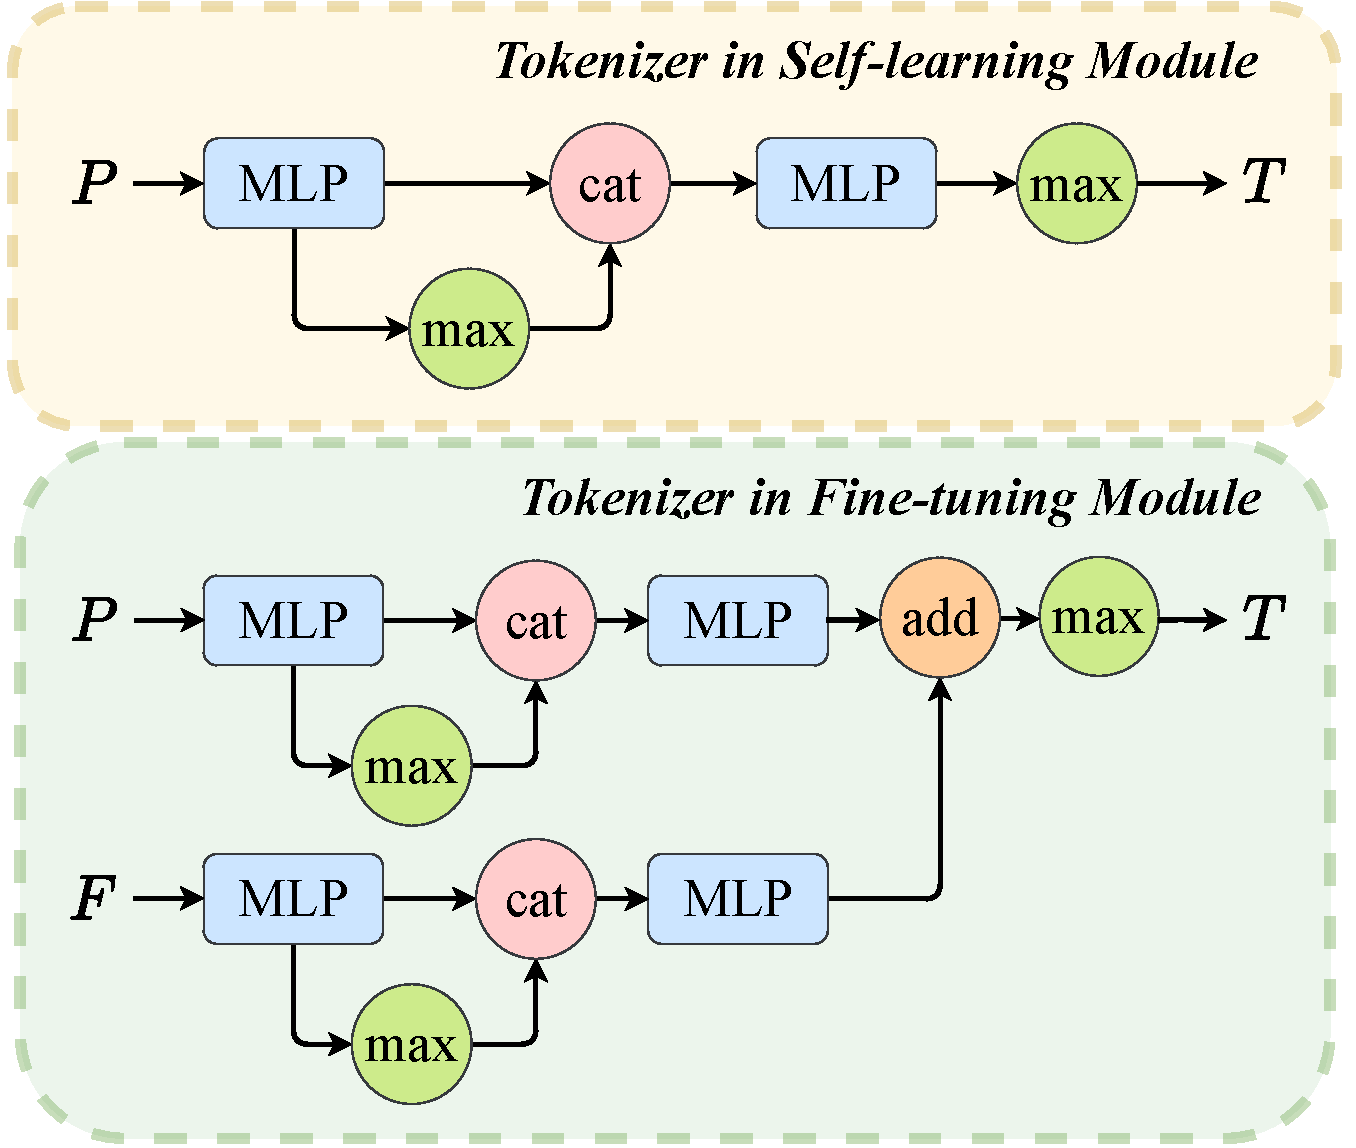
\includegraphics[width=1\columnwidth]{sup_pic/tokenizer_new.drawio.pdf}
    \caption{The network design details for the tokenizer. The primary distinction between the tokenizer in the fine-tuning module and that in the self-learning module lies in the integration of the motion flow features, denoted as $F$. } 
    \label{fig:tokenizer}
    \vspace{-1ex}
\end{figure}
As previously mentioned, in the self-learning module, the motion flow features $F$ are not fused with the part patches features $P$. This design prevents premature leakage of location information of masked tokens to the STEncoder.  
The network design details for the Tokenizer are illustrated in Figure.~\ref{fig:tokenizer}. 
During self-learning, each point of $P$ is mapped to a feature vector using several shared MLPs. Subsequently, max-pooled features are concatenated to each feature vector. These are then processed through several MLPs to expand their dimension to $C=384$. 
During fine-tuning, the same operation is applied to the motion flow $F$. The features of $P$ and $F$ are then fused through element-wise addition. Finally, a max-pooling layer is applied to derive the part token $T$. 


\begin{table}[ht]
\centering
\caption{Comparative Analysis of Model Parameter Numbers in Transformer-Based Dynamic Point Cloud Methods.}
\begin{tabular}{l|cc}
\Xhline{1px}
                                                          & \multicolumn{2}{c}{Num of Params(M)$\downarrow$}            \\ \hline
                                                          & \multicolumn{1}{c|}{Self-learning} & Fine-tuning \\ \hline
P4Transformer~\cite{fan2021point}   & \multicolumn{1}{c|}{/}             & 40.37       \\ \hline
PST-Transformer~\cite{fan2022point} & \multicolumn{1}{c|}{/}             & 60.36       \\ \hline
PPTr~\cite{wen2022point}            & \multicolumn{1}{c|}{/}             & 120.7       \\ \hline
MaST-Pre~\cite{shen2023masked}      & \multicolumn{1}{c|}{140.76}        & 120.66      \\ \hline
UniPVU-Human                                              & \multicolumn{1}{c|}{\textbf{34.92}}         & \textbf{22.48}       \\ \Xhline{1px}
\end{tabular}
\label{tab:model_size}
\end{table}


\section{Supplementary Comparison Experiments on HuCenLife~\cite{xu2023human}}
For more comprehensive and extensive comparisons, we supplement our comparison experiments on HuCenLife~\cite{xu2023human} with methods specifically designed for modeling dynamic point cloud videos~\cite{fan2022pstnet,fan2021point,fan2022point,wen2022point,fan2021deep}. As can be seen from Table.~\ref{tab:sup_comp_exp}, although these methods perform better in categories that require modeling motion features for accurate recognition (Fitness, Sports, Bend-Over, Walk-Stand) than static point cloud methods, there is still a significant performance gap compared to our UniPVU-Human. This confirms the superiority of our method in capturing human motion representations. We also compared our method with self-learning approaches based on contrastive learning~\cite{shen2023pointcmp}. The experimental results demonstrate the superiority of our self-learning mechanism.


\section{Comparative Analysis of Model Parameter Numbers}
Transformer\cite{vaswani2017attention}-based methods~\cite{chen2023pointgpt,liu2023point,zhao2021point,guo2021pct} have achieved considerable performance in point cloud feature extraction. However, their large model size typically results in significant computational demands. As we can see from Table.~\ref{tab:model_size}, the parameter number of other transformer-based dynamic point cloud methods~\cite{fan2021point,fan2022point,wen2022point, shen2023masked}, are several times greater than that of our UniPVU-Human. Our model maintains a parameter number of twenty to thirty million in both the self-learning and fine-tuning stages, which is comparable to ResNet-50~\cite{he2016deep}. Therefore, our UniPVU-Human achieves better performance with fewer parameters, making it a lightweight and effective model well-suited for real-world applications. 


\end{appendix}

% \section{Rationale}
% \label{sec:rationale}
% % 
% Having the supplementary compiled together with the main paper means that:
% % 
% \begin{itemize}
% \item The supplementary can back-reference sections of the main paper, for example, we can refer to \cref{sec:intro};
% \item The main paper can forward reference sub-sections within the supplementary explicitly (e.g. referring to a particular experiment); 
% \item When submitted to arXiv, the supplementary will already included at the end of the paper.
% \end{itemize}
% % 
% To split the supplementary pages from the main paper, you can use \href{https://support.apple.com/en-ca/guide/preview/prvw11793/mac#:~:text=Delete%20a%20page%20from%20a,or%20choose%20Edit%20%3E%20Delete).}{Preview (on macOS)}, \href{https://www.adobe.com/acrobat/how-to/delete-pages-from-pdf.html#:~:text=Choose%20%E2%80%9CTools%E2%80%9D%20%3E%20%E2%80%9COrganize,or%20pages%20from%20the%20file.}{Adobe Acrobat} (on all OSs), as well as \href{https://superuser.com/questions/517986/is-it-possible-to-delete-some-pages-of-a-pdf-document}{command line tools}.